\chapter{Results}

\fancyhead[L]{Chapter 3: Results}
\fancyfoot[C]{\thepage}

\section{Overview of Model Output}
    \subsection{Baseline Simulations}
        \subsubsection*{Scenario 1: Standard Conditions}
        Initial model results show that under baseline conditions, key output parameters such as maximum system height reach a plateau at specific ranges of input values (see Figure \ref{fig:baseline_results}). For high input rates, the system exhibits instability, leading to non-linear behaviors. In contrast, empirical models predict a continuous increase in system response, which is not observed in our simulations due to limiting factors such as resource availability or energy dissipation.

        \subsubsection*{Scenario 2: Modified Parameters}
        Modifications to system inputs, such as introducing external factors, reveal significant deviations from baseline results. For example, introducing external variables produces enhanced outcomes at lower input rates but suppresses system performance at higher rates. Figure \ref{fig:modified_conditions} illustrates the divergence in behavior across varying conditions.
    
    % \begin{figure}[h!]
    %     \centering
    %     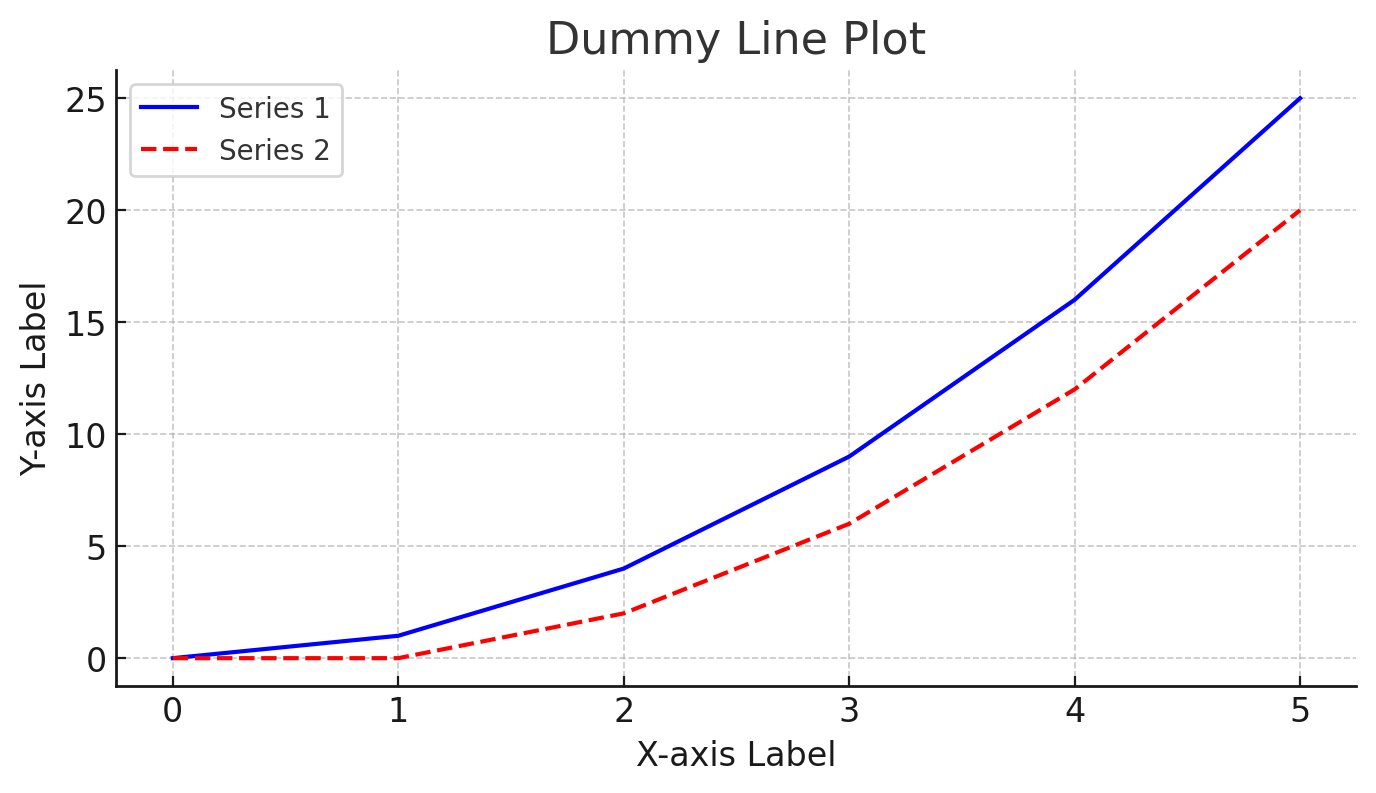
\includegraphics[width=150mm,scale=0.9]{placeholder_image1.png}
    %     \caption[Baseline Simulation Results]{Baseline simulation results showing the relationship between input parameters and system output under standard conditions.}
    %     \label{fig:baseline_results}
    % \end{figure}

\section{Impact of External Factors}
    \subsection{Effect on System Dynamics}
    To quantify the influence of external variables, we analyze the change in output relative to baseline conditions:
    \begin{equation}\label{delta_output}
        \Delta R = R_{external} - R_{baseline}
    \end{equation}
    where $R_{external}$ represents the system response with external factors, and $R_{baseline}$ represents the baseline response. Figure \ref{fig:delta_response} visualizes these variations, highlighting distinct regions of system enhancement or suppression.

    % \begin{figure}[h!]
    %     \centering
    %     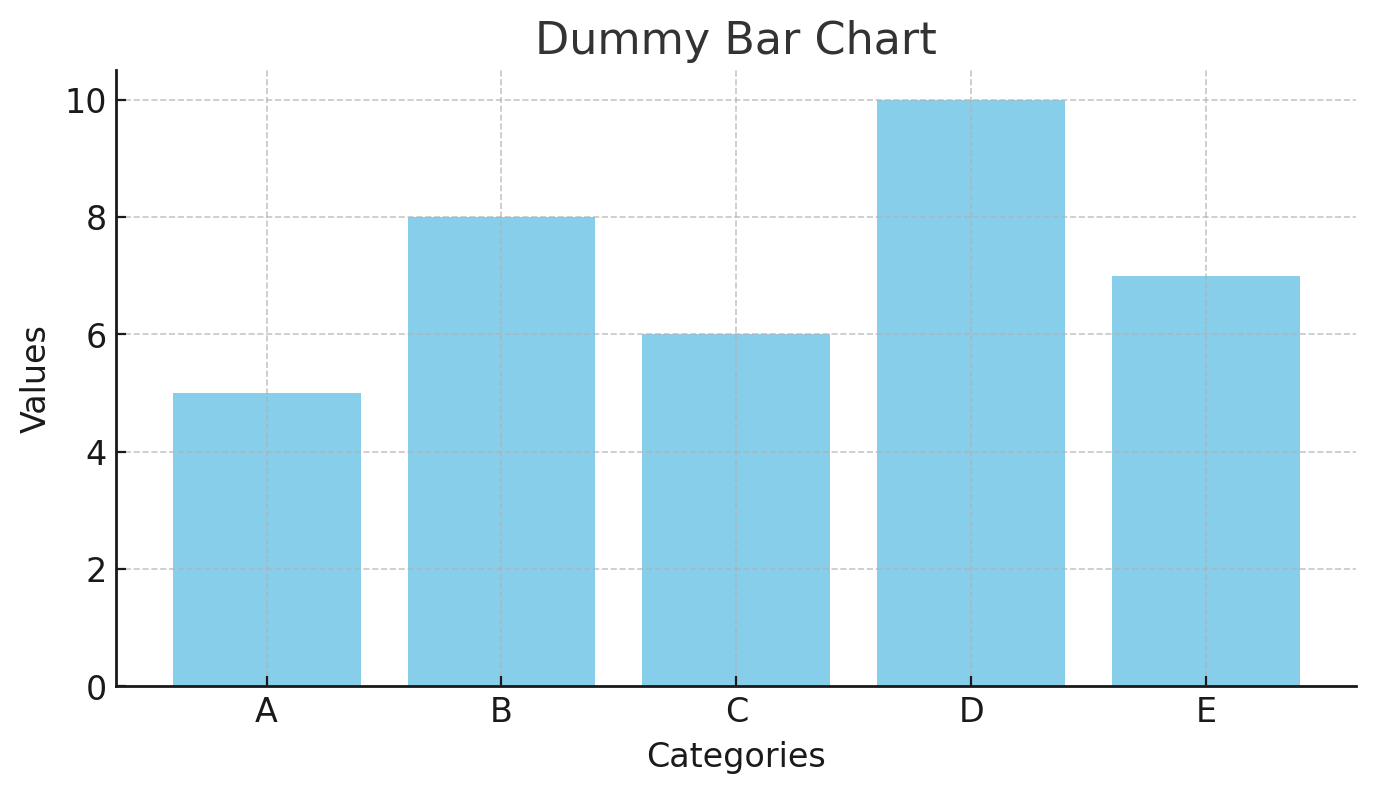
\includegraphics[width=150mm,scale=0.9]{placeholder_image2.png}
    %     \caption[Change in System Response]{Change in system response ($\Delta R$) as a function of external input levels and baseline conditions.}
    %     \label{fig:delta_response}
    % \end{figure}

    \subsection{Regional Variations in System Behavior}
    Analysis reveals four primary response regimes based on external input levels:
    \subsubsection*{Region 1: Minimal Impact}
    In this regime, external factors produce a small decrease in output, typically less than 10\%. Input values are moderate, and external contributions remain below critical thresholds.

    \subsubsection*{Region 2: Significant Suppression}
    This regime is characterized by a marked decline in output, up to 50\%, due to high external input levels. Threshold values are exceeded, leading to destabilization of system dynamics.



\section{Statistical Analysis of Results}
    A histogram of output variations (Figure \ref{fig:histogram_results}) illustrates the distribution of changes across all scenarios. Key trends include a clustering of minor changes around baseline conditions and a secondary peak indicating significant enhancements.

    % \begin{figure}[h!]
    %     \centering
    %     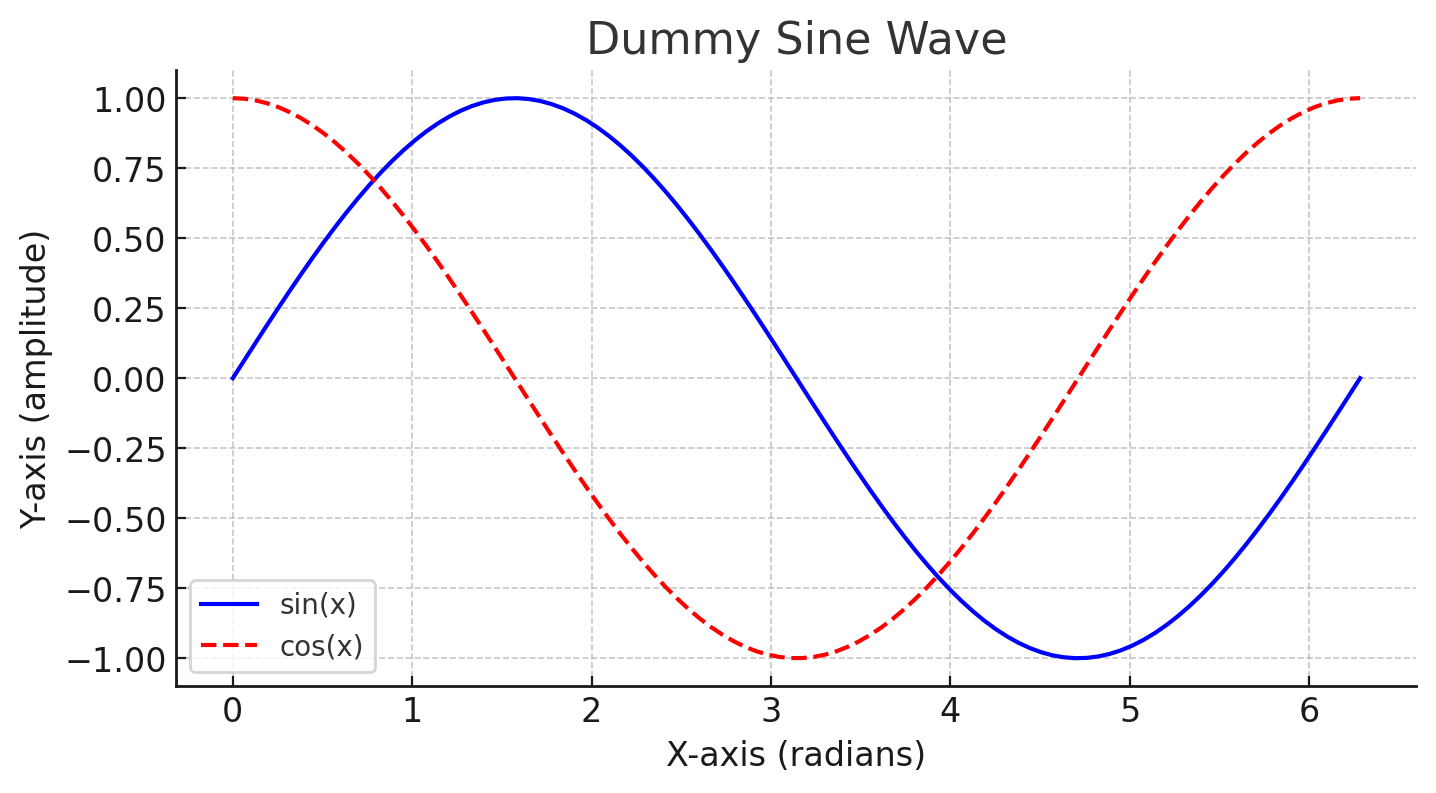
\includegraphics[width=150mm,scale=0.9]{placeholder_image4.png}
    %     \caption[Distribution of Output Variations]{Histogram showing the distribution of output variations across all simulated scenarios.}
    %     \label{fig:histogram_results}
    % \end{figure}

\section{Key Findings and Insights}
    The results of this study demonstrate:
    \begin{enumerate}
        \item System behavior is highly sensitive to input parameters, particularly at extreme values.
        \item External factors can both enhance and suppress system performance depending on input ranges.
        \item Optimizing input levels can lead to significant performance gains while avoiding destabilization.
    \end{enumerate}

    These findings provide a framework for further exploration of parameter sensitivities and inform strategies for system optimization.
